\documentclass[a0,landscape]{a0poster}
% Постер по проекту: чистый безрамочный 3-колоночный стиль
% (красный заголовок, синие заголовки секций с линейкой, белый фон)
% в духе шаблона optimization-class poster. Содержание согласовано
% с финальной refactored_paper.tex: фильтры F0–F5 (включая каскад F5),
% шумы N1–N4, 100 сидов, стат-критерии (Макнемар, two-stage, TOST,
% кластерный бутстрап), блочный дизайн.

\usepackage{fontspec}
% Кириллицу XeLaTeX берёт прямо из шрифта; polyglossia не используем, т.к.
% масштабирование шрифтов в a0poster (a0size) ломает её проверку OpenType.
\setmainfont{PT Sans}
% мягкие переносы недоступны без polyglossia — снимаем переполнения строк
\tolerance=2000
\emergencystretch=3em
\sloppy

\usepackage{amsmath,amssymb}
\usepackage{multicol}
\usepackage{graphicx}
\usepackage{booktabs}
\usepackage{array}
\usepackage{xcolor}

\definecolor{titlered}{RGB}{170,30,30}
\definecolor{headblue}{RGB}{0,71,133}

\setlength{\columnsep}{3cm}
\setlength{\parindent}{0pt}
\setlength{\parskip}{0.7\baselineskip}

% синий заголовок секции с линейкой — как в шаблоне
\newcommand{\heading}[1]{\bigskip{\color{headblue}\LARGE\bfseries #1}\par
  \vspace{0.2\baselineskip}{\color{headblue}\hrule height 1.4pt}\medskip}

\newcommand{\R}{\mathbb{R}}
\newcommand{\E}{\mathbb{E}}
\newcommand{\norm}[1]{\lVert#1\rVert}
\DeclareMathOperator{\med}{med}

\begin{document}

% ===================== ШАПКА =====================
{\color{titlered}\veryHuge\bfseries
Beyond Gaussian Noise: Convergence of Stochastic Optimizers\\
under Correlated and Heavy-Tailed Financial Gradient Noise\par}
\medskip
{\Large Д.~Кортунов \quad В.~Пастушенко \quad А.~Дубовицкий \quad А.~Шадрин\par}
\smallskip
{\Large\textit{НИУ ВШЭ, Москва}\par}
\medskip
{\color{titlered}\hrule height 3pt}
\bigskip

\begin{multicols}{3}

% ----------------------- КОЛОНКА 1 -----------------------
\heading{Постановка}
Наблюдаемый ряд~--- сигнал плюс шум, $y_t = s_t + \xi_t$. Перед обучением
весь ряд проходит через причинный фильтр $F$: $\tilde y = F(y)$, и уже
из сглаженного ряда строятся признаки $\tilde\phi_t$. Обучаем прогнозную
модель (AR($p$)) минимизацией риска методом первого порядка
\[
  g_k=\tfrac1{|\mathcal B_k|}\!\!\sum_{t\in\mathcal B_k}\!\!
      \nabla_x\ell(x_k,\tilde\phi_t,c_t),\qquad
  x_{k+1}=x_k-\eta\,\phi(g_k).
\]
Признаки и обучающий таргет~--- из ряда $\tilde y$; качество же
оценивается на holdout по исходному будущему значению $y_t$.

На финансовых рядах шум тяжёлохвостый ($\alpha$-устойчивый, $\alpha<2$,
бесконечная дисперсия) и долгопамятный. Тогда базовые предпосылки теории
сходимости SGD нарушаются.

\medskip
Вопрос. Как тройка
(тип шума)~$\times$~(фильтр)~$\times$~(оптимизатор) влияет на сходимость,
и можно ли по диагностике ряда заранее выбрать удачную пару?

\heading{Четыре класса шума}
\begin{tabular}{@{}ll@{}}
\toprule
N1 & гауссов белый (контроль)\\
N2 & розовый $1/f$ (долгая память)\\
N3 & $\alpha$-устойчивый (тяжёлый хвост)\\
N4 & смешанный (хвост $\cap$ память)\\
\bottomrule
\end{tabular}

\heading{Фильтры $F_0$–$F_5$ (все причинные)}
\begin{tabular}{@{}ll@{}}
\toprule
$F_0$ & без фильтрации (контроль)\\
$F_1$ & скользящее среднее (линейный)\\
$F_2$ & фильтр Калмана (линейный)\\
$F_3$ & вейвлет-порог (Добеши)\\
$F_4$ & причинная медиана (робастный)\\
$F_5$ & каскад $F_4{\to}F_3$ (для N4)\\
\bottomrule
\end{tabular}\par
\smallskip
Оптимизаторы: SGD, Clipped-SGD, Normalized-SGD, Adam, AdamW.
Дизайн~--- \textbf{блочный} (не полный перебор): Блок~A (SGD-семейство, все
шумы N1--N4; спасение сходимости) и Блок~B (Adam/AdamW, N2/N4; скорость).
Шумы N2 и N4 проходят оба блока. По \textbf{100} независимых запусков
на ячейку.

% ----------------------- КОЛОНКА 2 -----------------------
\heading{Предпосылки и гипотезы}
Гипотезы выведены из теории и зафиксированы \emph{до} экспериментов.
При $\alpha<2$ второй момент градиентного шума бесконечен~--- редкие
гигантские шаги не дают SGD стабилизироваться. Хвост выборочной медианы
окна $w$ имеет порядок $\alpha\lceil w/2\rceil$: при $w{=}9$ конечная
дисперсия уже при $\alpha>0.4$. Линейные фильтры $\alpha$-устойчивость не
убирают; долгую память лечит спектральное разреживание (вейвлет) или
адаптивный шаг (Adam).
\begin{itemize}\setlength{\itemsep}{0.2\baselineskip}
\item Гипотеза 1 (N3): медиана $F_4$ переводит SGD в сходящийся
      режим; линейные фильтры~--- нет.
\item Гипотеза 2 (N2): для Adam/AdamW вейвлет $F_3$ ускоряет
      сходимость сильнее линейных фильтров.
\item Гипотеза 3 (N4): ни один простой фильтр не снижает
      асимптотический уровень $\|\nabla f\|^2$.
\item Гипотеза 4 (N1): фильтрация нейтральна, медиана чуть хуже
      среднего.
\end{itemize}

\heading{Эксперимент 1: тяжёлые хвосты ($\alpha{=}1.2$, SGD)}
Без фильтра и с линейными $F_1,F_2,F_3$~--- почти нет сходимостей; причинная
медиана $F_4$~--- $100/100$, асимптотический уровень $\|\nabla f\|^2$
ниже в $22$–$161\times$.
\begin{center}\small
\begin{tabular}{@{}lcccc@{}}
\toprule
Задача & бин.\,$F_0$ & бин.\,$F_4$ & асимпт.\,$F_0$ & асимпт.\,$F_4$\\
\midrule
квадратичная  & 2/100   & 100/100 & 0.456  & 0.0047\\
логистическая & 0/100   & 100/100 & 0.0767 & 0.00048\\
авторегрессия & 100/100 & 100/100 & 0.0479 & 0.0022\\
\bottomrule
\end{tabular}
\end{center}
\begin{center}
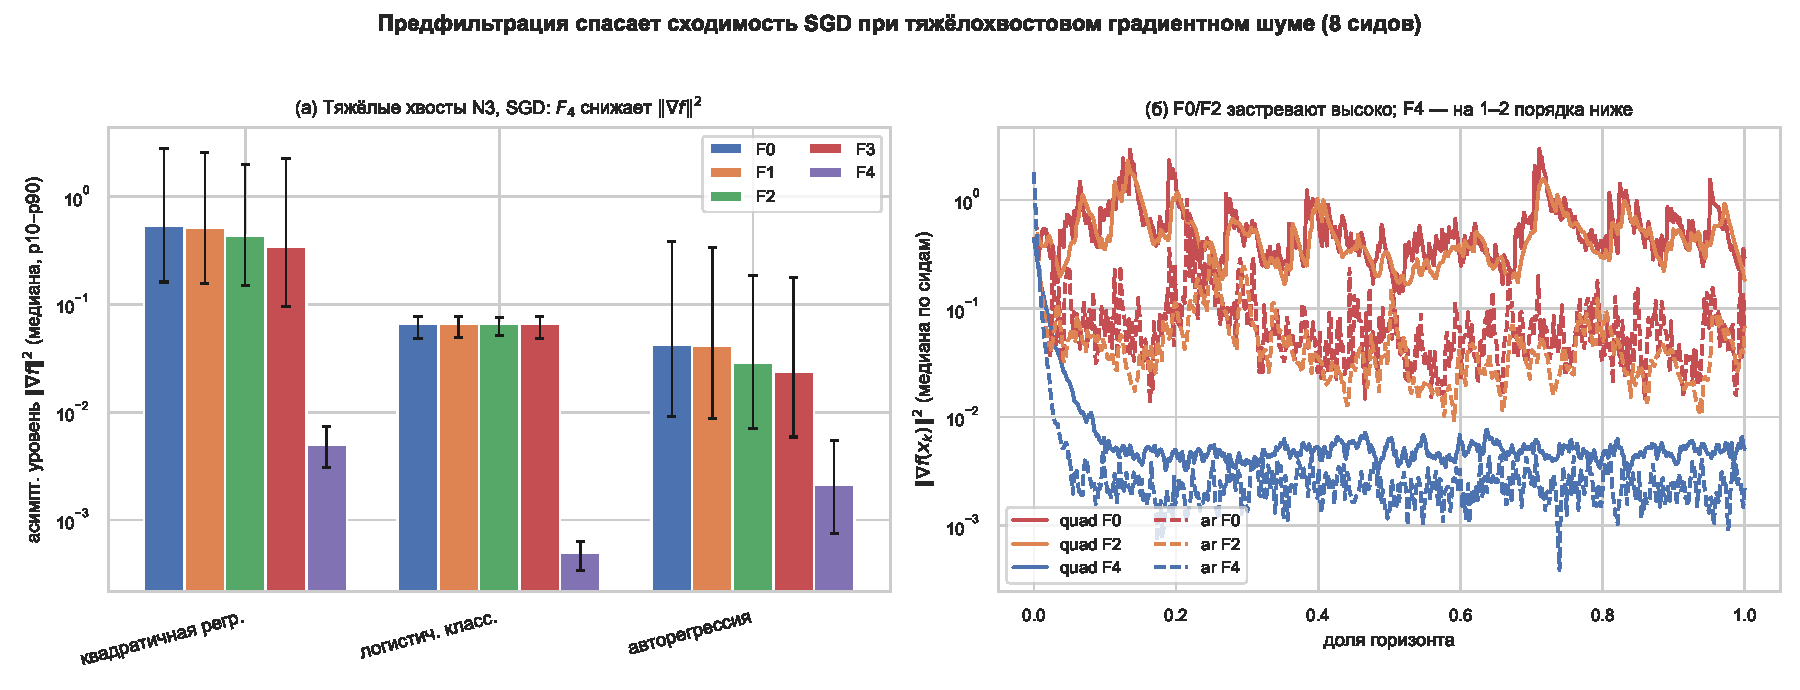
\includegraphics[width=\linewidth]{figures/convergence_rescue.pdf}
\end{center}
\vspace{-0.3\baselineskip}
{\small $F_0$ и линейные фильтры застревают на асимптотическом уровне;
$F_4$/$F_5$ уходят вниз на 1--2~порядка (6 фильтров, 100 сидов).}

\smallskip
Строгие критерии: парный $t$ на $\log_{10}\|\nabla f\|^2$~--- $d$~Коэна
$4.8$–$7.7$, $p_{\text{Холм}}{<}10^{-60}$, Стоуффер $Z{=}32.8$. Бинарную
сходимость проверяет точный критерий \textbf{Макнемара}
($0{\to}100/100$, $p{\approx}8{\times}10^{-31}$). Спасение устойчиво и под
Clipped-SGD ($3.2$–$5.2\times$).

% ----------------------- КОЛОНКА 3 -----------------------
\heading{Долгая память, смешанный шум, гауссов контроль}
N2, Adam: вейвлет $F_3$ ускоряет сходимость в
$4.9\times$ ($T_\varepsilon$ $814{\to}165$), Калман $F_2$~---
$1.9\times$; линейные, медиана и даже каскад $F_5$ ($0.9\times$)~--- нет.
\begin{center}
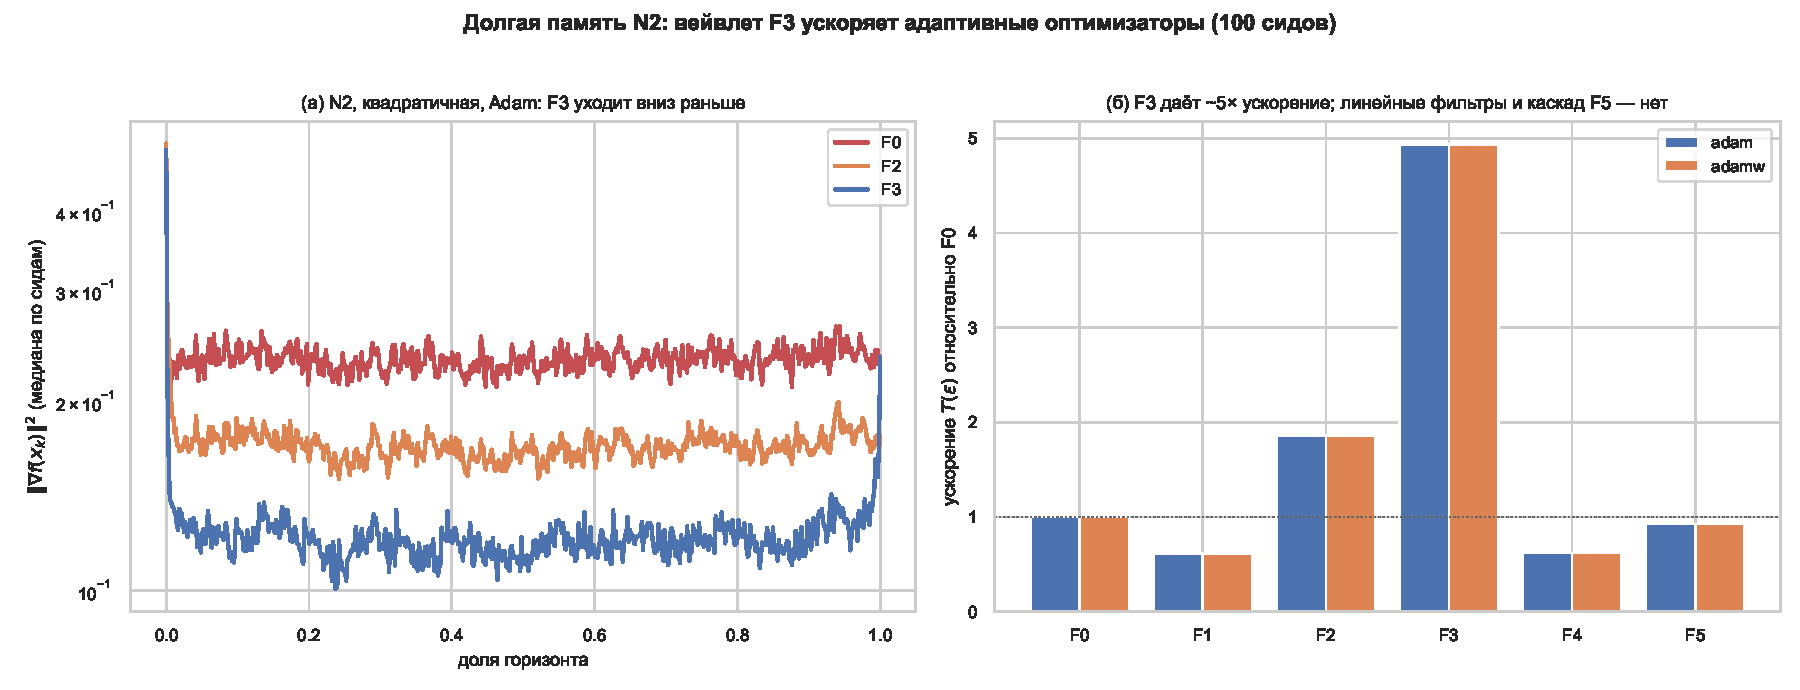
\includegraphics[width=\linewidth]{figures/longmemory_wavelet.pdf}
\end{center}
\vspace{-0.2\baselineskip}
N4: отношение асимптотических уровней $F_0/F_k\approx1$ для всех простых
фильтров \emph{и} двухстадийного каскада $F_5$~--- мешанный режим не
закрывается (гипотеза~3). N1: фильтрация нейтральна, $F_4$ слегка
проигрывает среднему (гипотеза~4); TOST подтверждает эквивалентность $F_0$:
\begin{center}
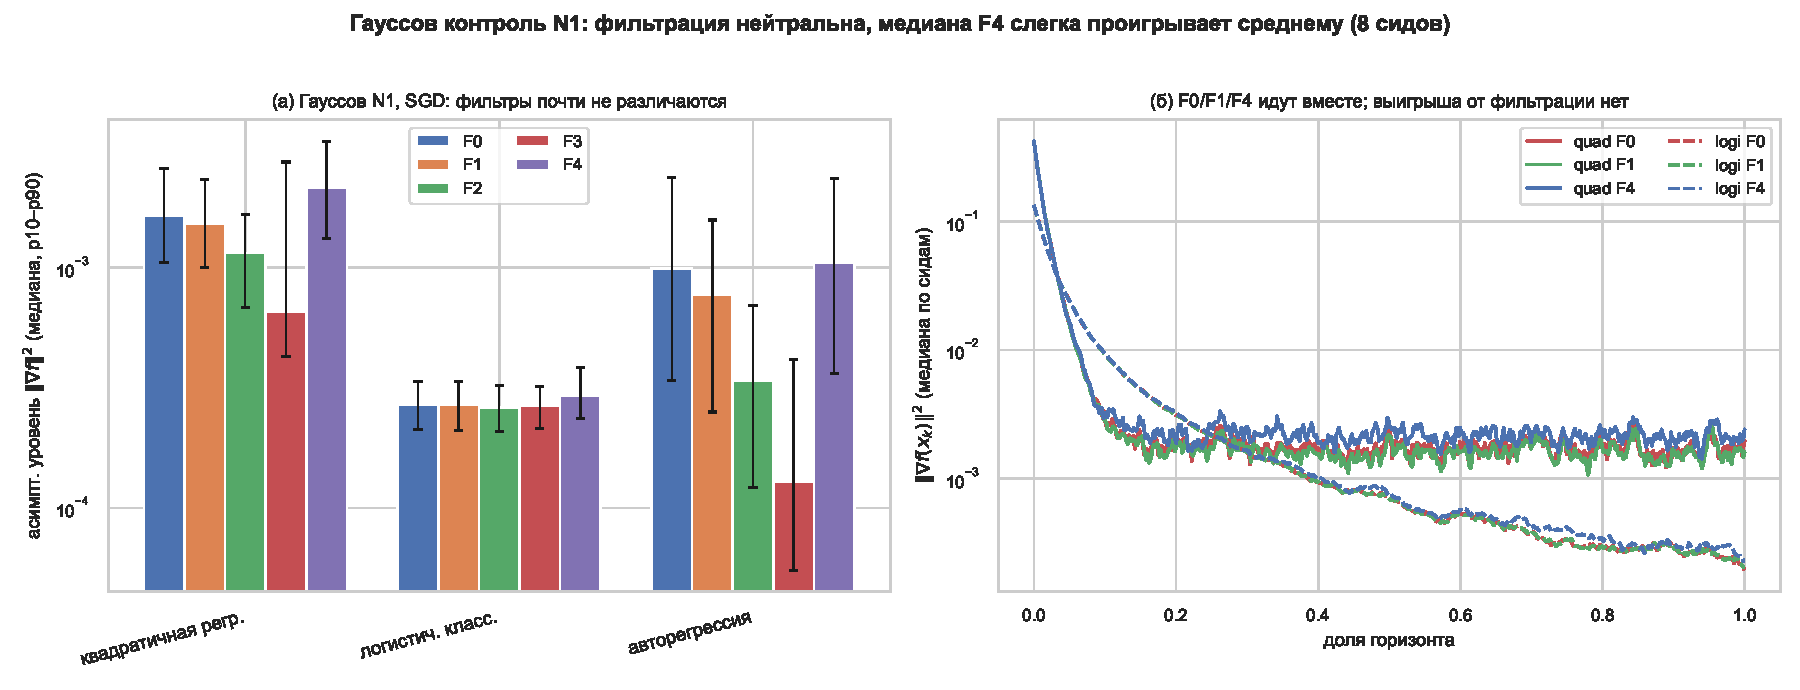
\includegraphics[width=\linewidth]{figures/gaussian_control.pdf}
\end{center}

\heading{Каскад $F_5$ для N4}
Двухстадийный каскад $F_5=F_4{\to}F_3$ (медиана против выбросов, затем
вейвлет против $1/f$-памяти) прогнан как полноправный фильтр. На N3 он даже
\emph{сильнее} простой медианы ($136$/$168$/$36\times$), но \textbf{N4 не
закрывает} (отношение уровней $1.0$–$1.2$, TOST: $F_4,F_5\equiv F_0$).

\heading{Эксперименты 2–3: калибровка и реальные ряды}
Медиана хвостов по корзине реальных инструментов: $\hat\alpha\!\approx\!1.21$,
$\hat d\!\approx\!0.29$. На калиброванной синтетике спасение сходимости
сохраняется ($91$–$129\times$):
\begin{center}
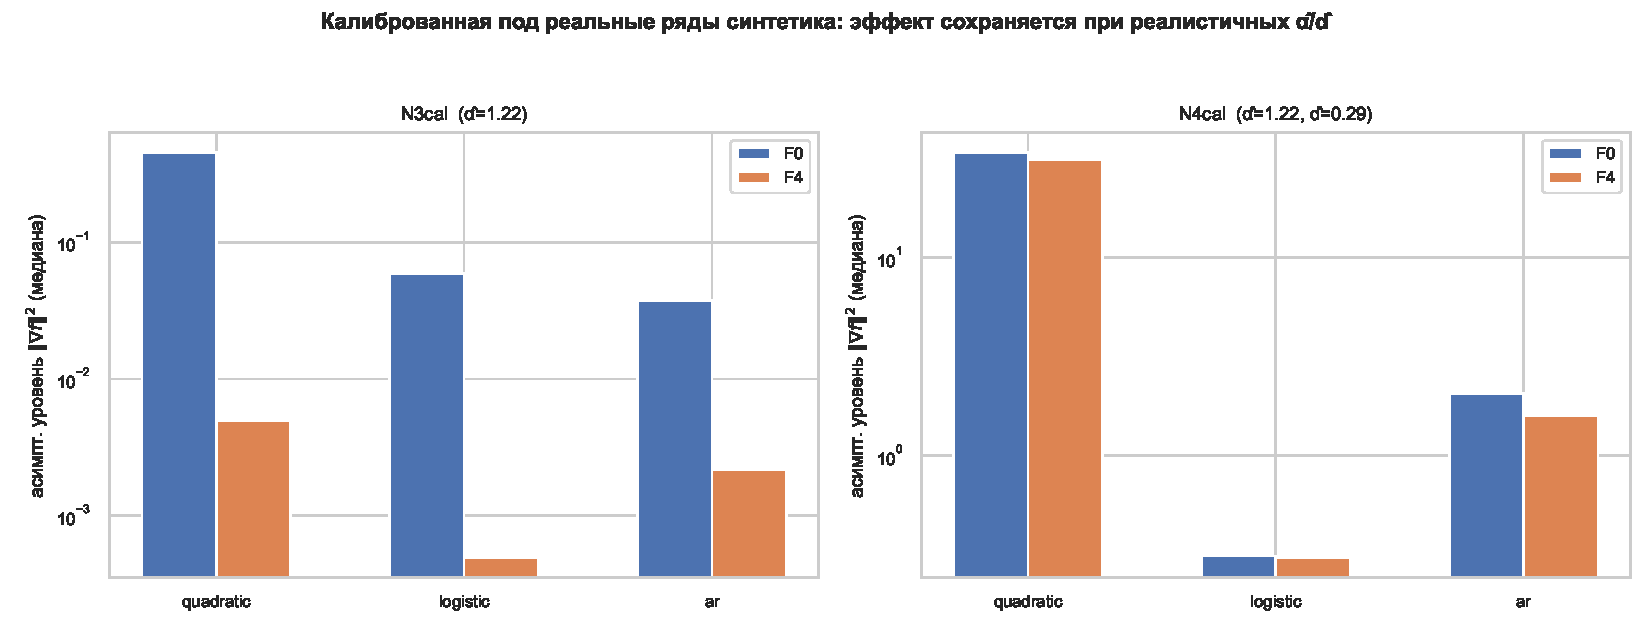
\includegraphics[width=\linewidth]{figures/calibrated_synthetic.pdf}
\end{center}
На реальных рядах (Adam) фильтр Калмана $F_2$ резко ускоряет сходимость:
\begin{center}\small
\begin{tabular}{@{}lcccc@{}}
\toprule
Домен & сошл.\,$F_0$ & лучший & ускор. & holdout (лучш./$F_0$)\\
\midrule
фин.\ 15-мин  & 109/200 & $F_2$ & $51\times$ & 0.529/0.522\\
фин.\ дневные & 322/400 & $F_2$ & $11\times$ & 0.635/0.626\\
сенсор ETT    & 100/100 & $F_1$ & $2.2\times$ & 0.641/0.488\\
макро FRED    & 300/300 & $F_0$ & ---        & $F_0$ лучший\\
\bottomrule
\end{tabular}
\end{center}
\textbf{Но скорость $\ne$ точность:} кластерный бутстрап по holdout-MSE
(ресэмпл рядов) показывает, что прогноз фильтр \emph{не} улучшает~---
доверительный интервал выше нуля на всех доменах. Фильтр~--- инструмент
кондиционирования оптимизации, а не улучшения прогноза.

\heading{Правило $(\hat\alpha,\hat H)\to$ фильтр}
\begin{center}\small
\begin{tabular}{@{}lll@{}}
\toprule
Режим $(\hat\alpha,\hat H)$ & связка & основание\\
\midrule
$\hat\alpha{\approx}2,\ \hat H{\approx}0.5$ & $F_0$ & теория+опыт\\
$\hat\alpha{\approx}2,\ \hat H{>}0.6$       & $F_3{+}$Adam & теория+опыт\\
$\hat\alpha{<}1.9,\ \hat H{\approx}0.5$     & $F_4{+}$SGD & теория+опыт\\
$\hat\alpha{<}1.9,\ \hat H{>}0.6$ (N4)       & нет рецепта & открытый вопрос\\
\bottomrule
\end{tabular}
\end{center}

\heading{Выводы}
\begin{itemize}\setlength{\itemsep}{0.25\baselineskip}
\item Робастная медиана восстанавливает конечную дисперсию градиента~---
линейные фильтры этого не дают.
\item Тяжёлый хвост сам по себе не повод фильтровать: если узкое
место не в сходимости (гаусс, светлый хвост), лучший выбор~--- $F_0$.
\item На реальных рядах фильтр ускоряет оптимизацию, но прогноз на holdout
не улучшает (и может ухудшить).
\item Каскад $F_5$ усиливает эффект на N3, но смешанный N4 остаётся открытым.
\item Все четыре гипотезы подтвердились на 100~сидах формальными
стат-критериями.
\end{itemize}

\vfill
{\small Код и данные: \texttt{github.com/Poogee/momo\_proj}}

\end{multicols}
\end{document}
